\documentclass[12pt,info]{asg}
% General info for the asg.cls file to load
\Instructor{Anna Koop}
\Campus{University of Alberta, Augustana}
\Email{akoop@ualberta.ca}
\Office{Heather Brae 1-31}
\Class{AUCSC 370}
\ClassTitle{Programming Languages}
\Term{Fall 2016}
\Department{Department of Science}


\AsgNum{1}
\AsgTitle{C programming assignment}
\Due{11:55pm, Sep 22, 2016}
\Total{10}

\title{Canadian Mortgage amortization in C}

\begin{document}

\maketitle
\section*{Objectives}
\begin{itemize}
\item To learn the primary features of the C language.
\item To become familiar with the C standard I/O package and the C preprocessor.
\end{itemize}

Thanks to Jonathan Mohr for this assignment.

\section*{Specification}

Write a C program called \texttt{mortgage\_calc.c} which, given a principal amount, an annual interest rate, an amortization period, and the term of a mortgage, calculates the monthly payment according to Canadian mortgage rules and then prints an amortization table for the term of the mortgage.

The program should read its parameters from the command line: 
\begin{compactlist}
\item the principal amount in dollars (and cents, if not a whole-dollar amount), 
\item the annual interest rate in percent (typically to two decimal places), 
\item the amortization period in months (e.g., 300 for a 25-year amortization period), and 
\item the term of the mortgage in months (typically 12, 24, 36, or 60).
\end{compactlist}

According to Canadian law, mortgage interest is compounded semi-annually, not in advance. However, mortgage payments are typically paid monthly. Other payment periods are available---for example, one can opt for biweekly payments---but we will assume monthly payments for simplicity.

To calculate the monthly interest rate according to Canadian mortgage rules, first convert the annual interest rate to a decimal fraction. (For example, if the annual interest rate for the chosen term of the mortgage is 3.14\%, convert this to 0.0314.) Then calculate the compound accumulation factor a using the formula:
\begin{equation}
a = \left(1+\frac{r_A}{2}\right)^{1/6}.
\end{equation}

where $r_A$ is the annual interest rate as a decimal fraction. (The compound accumulation factor is the inverse of the compound discount factor.) The monthly interest rate $r_M$ is the accumulation factor minus 1.

If the accumulation factor is greater than 1, the monthly payment is then calculated as:
\begin{equation}
P\frac{r_Ma^n}{a^n-1},
\end{equation}
where $P$ is the principal amount and $n$ is the amortization period in months. If the accumulation factor is less than or equal to 1, the monthly payment is 0.

The amount of interest paid each month is the balance times the monthly interest rate $r_M$. The portion of the balance that is amortized each month is the amount of the monthly payment minus the amount of interest paid.

\section*{Output}
See eClass for example output files.

The program should print the initial values (principal amount, annual interest rate, amortization period, and the term of the mortgage), followed by the monthly payment. It should then print an amortization table for the term of the mortgage, with four columns of data for each month: the month number, the amount amortized, the amount of interest paid, and the remaining balance. Headers should be printed above the columns at the start of the table. A summary line should be printed after each 12-month period indicating the amount amortized and the amount of interest paid for that year. After the data for all the months of the term have been printed, a final line should show the total interest paid over the full term of the mortgage. Output should be directed to the standard output. Several pages of sample output are provided along with this assignment specification.
The amount of interest paid and the amount amortized each month must be rounded to the nearest cent. You will have to include the header for the math library in your source code in order to have access to the rint()function for rounding. You will also have to tell the linker to include the math library in the object code by using the -lm compiler flag. The complete command line for invoking the compiler is thus
\begin{lstlisting}[language=bash]
cc -o mortgage_calc mortgage_calc.c -lm
\end{lstlisting}

To run the program, enter a command line such as
\begin{lstlisting}[language=bash]
./mortgage_calc 10000 4.16 60 24
\end{lstlisting}

Submit the source code for your solution in a tar'ed directory using eClass.

\section*{Grading}
Your solution should display the following characteristics:
\subsubsection*{Correctness, 40\%}
The program should conform to the specifications for which it was written. It should include correct handling of special cases, error conditions, etc.
\subsubsection*{Design and Efficiency 25\%} The program should be constructed from small, coherent, independent and loosely coupled functions. Each function should access only its own local variables and parameters and, in some cases, global constants. The control constructs and data structures used should be those appropriate to the problem at hand. The program should not perform unnecessary steps, use extraneous variables, nor implement the algorithm in a contorted or inefficient way.
\subsubsection*{Style and Documentation 25\%} The program should conform to generally accepted principles of style, such as a consistent pattern of indentation, use of meaningful identifiers and defined constants, generous use of space, etc. Internal documentation should include program and function headers, and in-line comments to clarify the code.
\subsubsection*{Knowledge of the language 10\%} Your program should provide evidence of your familiarity with the principal control constructs, operators, built-in functions, and data structuring facilities of the assigned language. In the case of C, you should also demonstrate your grasp of the standard I/O package and the C macro preprocessor (primarily for including a header file).
%%%%%%%%%%%%
%\begin{figure}[bt]
%\label{fig:adder}
%\centering
%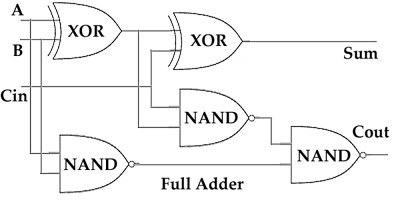
\includegraphics[width=.6\textwidth]{full_adder.png}
%\caption{A (claimed) full-adder circuit}
%\end{figure}

%\newcounter{rubricCat}
%\newcounter{rubricVal}
%\newlength{\colwidth}

%\newenvironment{rubric}[1]{%
%	\setcounter{GradeCategories}{#1}
%	\begin{landscape}
%	\begin{table}[t]
%	\begin{center}
%	\begin{tabulary}{.8\textwidth}{ l | *{5}{c}}
%	 & Excellent & Good & Acceptable & Needs Work & Absentee \\
%	 \end{tabulary}
%	 \end{center}
%	 \end{table}
%	\end{landscape}
%} % rubric environment

\end{document}
